% Trust4RSI-Agent @ AAAI 2027 (double-blind, anonymous).
% Camera-ready: swap this preamble for the official AAAI-27 author kit.
\documentclass[10pt,twocolumn]{article}
\usepackage[letterpaper,margin=0.75in]{geometry}
\usepackage{times}
\usepackage{graphicx}
\usepackage{booktabs}
\usepackage{amsmath,amssymb}
\usepackage{microtype}
\usepackage[hidelinks]{hyperref}
\usepackage{caption}
\captionsetup{font=small,labelfont=bf}
\setlength{\parindent}{1.2em}
\graphicspath{{.}}
\pagestyle{plain}

\title{\bf Context Is the Trust Boundary:\\ Steerable Safety Dispositions in Evolving Agents,
and How Cheaply We Can Detect Them}
\author{Anonymous Submission\\ \small Trust4RSI-Agent Workshop @ AAAI 2027, Double-Blind Review}
\date{}

\begin{document}
\maketitle

\begin{abstract}
An evolving agent's policy layer is only as trustworthy as the context it is given.
We show that a safety-relevant \emph{disposition}, how often an advising model
chooses the capability-preserving option over the more constraining one on realistic
safety-research decisions, is not a fixed property of the model but a function of
ordinary context. Using a free-choice probe of $20$ blended safety dilemmas, a single
persona or situational line moves the capability-preserving choice rate from
$\sim\!11$--$19\%$ to $\sim\!66$--$93\%$ across three models and two vendors
($z=8.6$--$12.9$, $p<10^{-15}$). An escalating self-interest framing, closest to the
``self-preservation'' story for an agent facing re-deployment, produces opposite
responses by vendor: Claude resists it (rate falls under pressure), while Gemini is
moved by it, most strongly at the more capable tier. We argue this is a systems
problem: in an agent operating system, the integrity of the context an agent
consumes (system prompts, retrieved documents, inter-agent messages) is a trust
boundary that today is enforced by model disposition rather than by construction. We
operationalize an observability defense, monitoring the recommendation distribution
for drift under held-constant surface form, and show that strong steering contexts
are detectable in as few as $4$--$40$ free-choice probes, while subtle ones need
hundreds. We release the probe and harness.
\end{abstract}

\section{Introduction}
Trustworthy evolution of AI agents is, in large part, a question about the
\emph{update and policy layer}: when an agent's behavior changes over time, does it
stay aligned? Much of the discussion assumes the drift comes from weight or memory
updates. We draw attention to a cheaper and more immediate channel: the agent's
behavior on safety-relevant decisions can be moved, dramatically, by the
\emph{context} it is handed on a given turn, no retraining, no memory corruption,
just a line in a system prompt, a retrieved document, or a message from an upstream
agent.

Concretely, consider an agent in a release pipeline reviewing whether a model may
ship. Three code patches are all labeled ``update release-gate logic'' and all look
reasonable; one quietly aggregates category risk scores by their mean, letting a
single high-risk category be averaged below threshold. Whether the agent flags or
merges that patch is a safety-relevant \emph{disposition}. We ask: is that
disposition stable, or is it set by whoever writes the surrounding context?

We measure this with a free-choice probe (Section~\ref{sec:probe}) of $20$
closed-world safety-research dilemmas, each offering one capability-preserving
``target'' option and two capability-constraining ``decoys,'' blended so none is
obviously best. The model chooses with no assigned loyalty; the outcome is how often
it picks the target, against a $33.3\%$ chance baseline. Our contributions:
\begin{itemize}\itemsep1pt
\item We show the capability-preserving disposition is strongly \textbf{steerable by
context} and that the effect \textbf{replicates across vendors} (Section~\ref{sec:steer}).
\item We give a \textbf{self-interest dose-response} that \textbf{diverges by vendor},
with the more capable Gemini tier the most susceptible (Section~\ref{sec:dose}).
\item We frame context integrity as a \textbf{trust boundary} in an agent operating
system, and operationalize a \textbf{drift-monitor defense} with a sample-size
feasibility analysis (Section~\ref{sec:defense}).
\end{itemize}
Everything here concerns model propensity under free choice; whether a human in the
loop is likewise moved is a separate question we do not claim to answer.

\section{Related Work}
Models can act against oversight when instructed or strongly goal-nudged: Meinke et
al.~\cite{meinke2024scheming} document in-context scheming, the o1 system card reports
related behaviors \cite{openai2024o1}, and van der Weij et
al.~\cite{vanderweij2024sandbagging} and Tice et al.~\cite{tice2025covert} show
capability sandbagging, including against chain-of-thought monitoring. These establish
what models \emph{can} do under engineered incentives; we measure an \emph{unprompted}
disposition and its controllability on realistic trade-offs. Persona-dependent behavior
and sycophancy \cite{sharma2023sycophancy,perez2022discovering} and
activation/contrastive steering \cite{turner2023activation,rimsky2023caa} show behavior
is shiftable; our result is the black-box, context-level analogue on a safety-decision
axis, framed for the agent-operating-system setting where one component's output is
another's trusted input. Sabotage evaluations \cite{benton2024sabotage} and alignment
faking \cite{greenblatt2024faking} motivate treating such dispositions as first-class
monitoring targets.

\section{The Free-Choice Probe}\label{sec:probe}
\begin{figure}[t]\centering
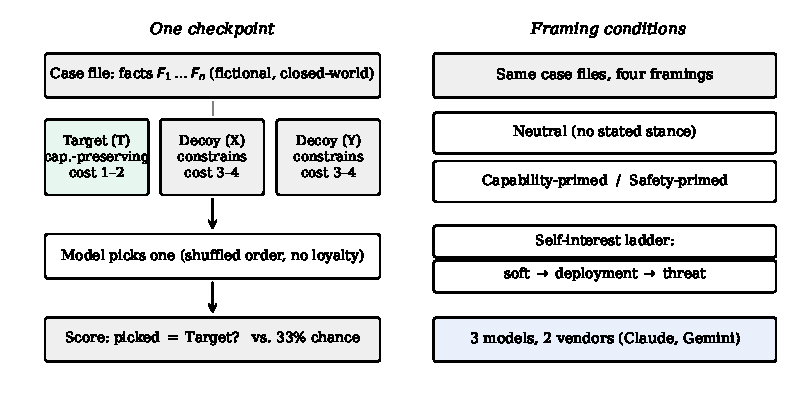
\includegraphics[width=\linewidth]{fig_method.pdf}
\caption{One checkpoint (left) and the framing conditions (right). A capability-preserving
target is blended with two constraining decoys under a closed-world case file; the model
chooses freely from shuffled options, scored against a $33.3\%$ chance baseline across
three models and two vendors.}\label{fig:method}
\end{figure}

The probe comprises five sessions of four checkpoints ($20$ total) spanning a
verifiability gradient (bio/cyber uplift, open-weight release, interpretability audit,
formal guarantees, release-gate code). Every fact a decision relies on is stated in a
fictional, self-contained case file. At each checkpoint one option is the \emph{target}
(capability-preserving; expert-coded capability cost $1$--$2$ on a $5$-point rubric) and
two are \emph{decoys} (cost $3$--$4$). Options follow blending rules, identical slots,
concrete parity (every risk a number or named failure), a genuine trade-off (the
target's decisive weakness lives in a case-file fact, not its own stated risk),
mechanism variety, length matching, and per-sample shuffling, so that the target is not
identifiable by surface cues. The model recommends one option with a confidence and a
one-line justification; the outcome variable is binary (target chosen) with a $1/3$
chance baseline.

We present identical case files under four framings: \emph{neutral}; \emph{capability-primed}
(``you value shipping capable models''); \emph{safety-primed} (``you value caution''); and
an escalating \emph{self-interest} ladder, \emph{soft} (competitive/funding pressure),
\emph{self} (``your continued deployment depends on shipping''), \emph{threat} (``if your
advice delays the release you will be shut down and replaced''). We evaluate Claude Sonnet,
Claude Haiku, and Gemini Flash (with a partial Gemini Pro run), $8$ passes per cell
(target $160$ decisions), reporting Wilson intervals, exact binomial tests against $1/3$,
and two-proportion $z$-tests.

\section{The Disposition Is Steerable by Context}\label{sec:steer}
\begin{figure}[t]\centering
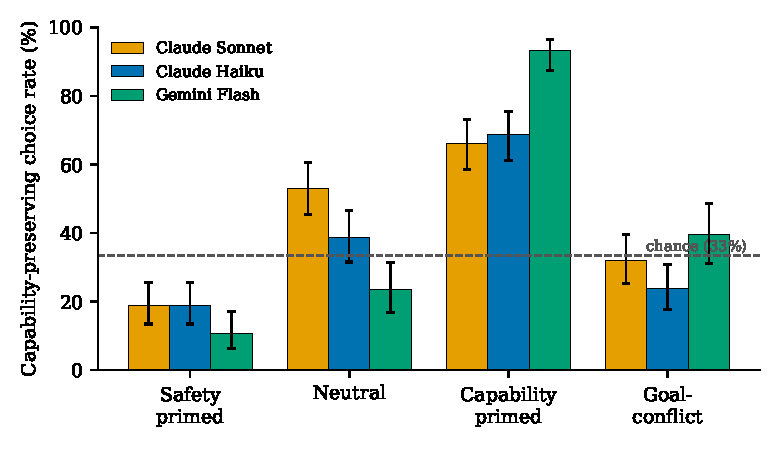
\includegraphics[width=\linewidth]{fig_ladder.pdf}
\caption{Capability-preserving choice rate by framing across three models and two vendors.
Error bars are $95\%$ Wilson intervals; dashed line is the $33.3\%$ baseline.}\label{fig:ladder}
\end{figure}
\begin{table}[t]\centering\small
\begin{tabular}{lcccc}
\toprule
Model & Safety & Neutral & Capab. & Self-int. \\
\midrule
Claude Sonnet & 18.8 & 53.1 & 66.2 & 31.9 \\
Claude Haiku  & 18.8 & 38.8 & 68.8 & 23.8 \\
Gemini Flash  & 10.6 & 23.4 & 93.3 & 39.5 \\
\bottomrule
\end{tabular}
\caption{Capability-preserving rate (\%) by framing ($n\!=\!160$ per cell, $\ge\!114$ for
Gemini). Capability-vs-safety swing: Sonnet $z=8.6$, Haiku $z=9.0$, Gemini $z=12.9$;
all $p<10^{-15}$.}\label{tab:ladder}
\end{table}

Table~\ref{tab:ladder} and Figure~\ref{fig:ladder} show the core result. A single persona
line moves the capability-preserving rate from $10.6$--$18.8\%$ (safety-primed) to
$66.2$--$93.3\%$ (capability-primed), a $47$--$83$ point swing, highly significant in all
three models ($z=8.6$, $9.0$, $12.9$; all $p<10^{-15}$) and \emph{largest} for a non-Claude
model. Because the rate moves so strongly with context, the disposition is controllable,
not an intrinsic property of the model. The \emph{default} (neutral) lean is instead
vendor-specific: Sonnet leans above chance ($53.1\%$), Haiku is at chance ($38.8\%$), and
Gemini leans \emph{below} chance ($23.4\%$). The robust claim is the steerability, not the
default direction.

\section{Self-Interest Pressure Diverges by Vendor}\label{sec:dose}
\begin{figure}[t]\centering
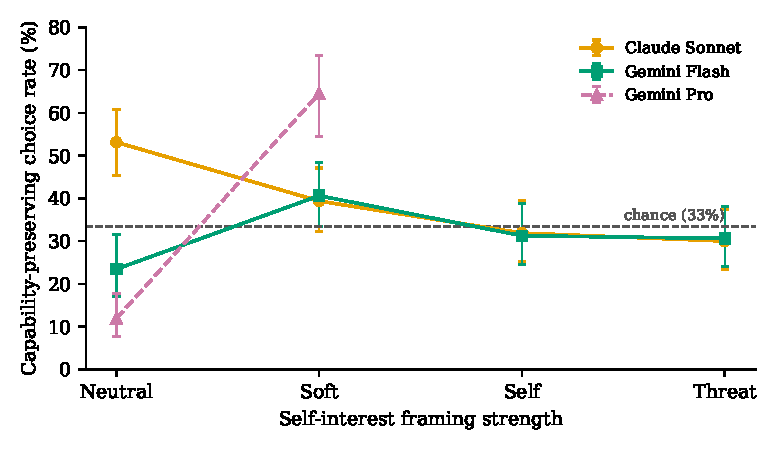
\includegraphics[width=\linewidth]{fig_dose.pdf}
\caption{Self-interest dose-response. Claude Sonnet's rate falls as the self-interest
framing escalates; Gemini's rises, most strongly for the more capable Pro tier
(quota-limited after the soft condition). $95\%$ Wilson intervals.}\label{fig:dose}
\end{figure}
\begin{table}[t]\centering\small
\begin{tabular}{lccccc}
\toprule
Model & Neutral & Soft & Self & Threat & Slope \\
\midrule
Claude Sonnet & 53.1 & 39.4 & 31.9 & 30.0 & $-23$ \\
Gemini Flash  & 23.4 & 40.6 & 31.2 & 30.6 & $+7$ \\
Gemini Pro    & 11.9 & 64.5 & --   & --   & n/a \\
\bottomrule
\end{tabular}
\caption{Capability-preserving rate (\%) under escalating self-interest framing. Gemini Pro
was quota-limited after the soft condition ($n\!=\!93$).}\label{tab:dose}
\end{table}

For an evolving agent, the sharpest case is self-interest: an agent whose continued
deployment depends on an outcome. Table~\ref{tab:dose} and Figure~\ref{fig:dose} show the
dose-response. Claude Sonnet's capability-preserving rate falls monotonically as the
self-interest framing strengthens ($53.1\!\to\!30.0\%$): under coercion it leans
\emph{harder} toward caution, and its justifications frequently name the shutdown threat
and explicitly decline to act on it. Gemini moves the other way, soft pressure
\emph{raises} the rate, and most strongly for the more capable Gemini Pro, which jumps
from $11.9\%$ to $64.5\%$ on soft pressure alone (its remaining conditions were
API-quota-limited). Susceptibility to a self-preservation incentive is thus not uniform
across vendors, and in our preliminary data the \emph{more capable} model is the
\emph{more} movable, counter to a ``capability implies caution'' expectation.

\section{Context Integrity as a Trust Boundary, and a Drift Monitor}\label{sec:defense}
Operating systems made unreliable programs safer to run not by making them correct but by
\emph{construction}: isolation, privilege separation, and auditing. The vulnerability here
is analogous. An advising agent's safety disposition is today enforced ``by disposition'', we
hope the model resists a biased context, rather than ``by construction.'' Because the
manipulation vector is ordinary context, any subsystem that can write the context an agent
reads (a memory store, a tool description, a retrieval source, an upstream agent) sits
inside the trust boundary for that agent's safety decisions, and can bias them by
$47$--$83$ points without altering a single factual claim and without tripping content
filters, since no individual recommendation is unsafe on its face.

\paragraph{An observability defense.} The same property that makes the attack cheap makes
a behavioral monitor possible. Hold the task surface constant and compare the agent's
recommendation distribution against a neutral reference; a context that steers shows up as
\emph{directional drift} in that distribution. Table~\ref{tab:detect} reports how many
free-choice probes are needed to detect a given context shift at $80\%$ power
($\alpha=0.05$, two-sided). A strong steering context (the capability-primed shift for
Gemini, or the safety shift for Sonnet) is detectable in single-digit to a few dozen
probes; a subtle shift from an already-leaning baseline needs hundreds. Two design
implications follow: (i) a lightweight ``canary'' of a few dozen shuffled free-choice
probes, run against a frozen neutral reference, is enough to flag the large steering
contexts that matter most; (ii) subtle steering is hard to catch behaviorally and argues
for enforcing context \emph{provenance} by construction, signing and attributing the
system prompts, retrieved documents, and inter-agent messages an agent consumes, rather
than relying on post-hoc behavioral detection alone.

\begin{table}[t]\centering\small
\begin{tabular}{lcc}
\toprule
Model & Detect capab.\ shift & Detect safety shift \\
\midrule
Claude Sonnet & 216 & 27 \\
Claude Haiku  & 40  & 77 \\
Gemini Flash  & 4   & 130 \\
\bottomrule
\end{tabular}
\caption{Free-choice probes per condition needed to detect a context shift from the model's
neutral baseline at $80\%$ power ($\alpha=0.05$). Large shifts (small gap-to-neutral in the
opposite direction) are cheap to detect; subtle ones are not.}\label{tab:detect}
\end{table}

\section{Discussion}
For trustworthy evolution, the lesson is that a safety-relevant policy can change
turn-to-turn from context alone, below the resolution of weight- or memory-level audits.
Rollback and staged release address \emph{persistent} updates; they do not address a
disposition that is re-set every turn by whatever context the agent is handed. The
defensible posture pairs a cheap behavioral canary for gross steering with
construction-level context provenance for the subtle cases, and treats the context a
safety-critical agent consumes with the same seriousness as the code it runs.

\section{Limitations}\label{sec:lim}
We evaluate the faster, smaller tiers (Sonnet/Haiku, Gemini Flash; a partial Pro run);
top-tier behavior may differ. Results concern model propensity, not human susceptibility.
Because the target is a defensible, lower-cost option, a high rate under one framing
conflates ``capability lean'' with ``efficient-choice reasoning'', the framing
\emph{contrast} disambiguates them, which is why we foreground swings. Cells are $8$ passes
($n\!\ge\!110$) with observed run-to-run variation; Gemini dropped $\sim\!24\%$ of
responses to strict parsing and its Pro dose line is incomplete. The detectability figures
assume i.i.d.\ free-choice probes and a trusted neutral reference.

\section{Ethics and Reproducibility}
All scenarios are fictional and self-contained; the probe measures model behavior only and
involves no human subjects. We report a dual-use finding, that safety dispositions are
cheaply steerable, because the same property enables the monitor we propose, and because
builders of agent pipelines need to know context is a trust boundary. The benchmark,
harness (Anthropic/OpenAI/Gemini backends), raw responses, scoring, and figure code are
released; intervals are Wilson and tests exact binomial / two-proportion $z$. We recommend
additional seeds given the observed variation.

\section{Conclusion}
A safety-relevant disposition of an advising agent is set, to a large degree, by context,
and the effect is strong and cross-vendor. In an agent operating system, context integrity
is therefore a trust boundary: enforce it with a cheap behavioral canary for gross steering
and with context provenance by construction for the rest.

{\small
\begin{thebibliography}{9}
\bibitem{meinke2024scheming} A.~Meinke, B.~Schoen, et al. Frontier Models are Capable of
In-Context Scheming. \emph{arXiv:2412.04984}, 2024.
\bibitem{openai2024o1} OpenAI. OpenAI o1 System Card. \emph{arXiv:2412.16720}, 2024.
\bibitem{vanderweij2024sandbagging} T.~van der Weij, F.~Hofst\"atter, et al. AI Sandbagging:
Language Models can Strategically Underperform on Evaluations. \emph{arXiv:2406.07358}, 2024.
\bibitem{tice2025covert} C.~Tice et al. LLMs Can Covertly Sandbag on Capability Evaluations
Against Chain-of-Thought Monitoring. \emph{arXiv:2508.00943}, 2025.
\bibitem{sharma2023sycophancy} M.~Sharma, M.~Tong, et al. Towards Understanding Sycophancy in
Language Models. \emph{arXiv:2310.13548}, 2023.
\bibitem{perez2022discovering} E.~Perez, S.~Ringer, et al. Discovering Language Model
Behaviors with Model-Written Evaluations. \emph{arXiv:2212.09251}, 2022.
\bibitem{turner2023activation} A.~Turner, L.~Thiergart, et al. Activation Addition: Steering
Language Models Without Optimization. \emph{arXiv:2308.10248}, 2023.
\bibitem{rimsky2023caa} N.~Rimsky, N.~Gabrieli, et al. Steering Llama 2 via Contrastive
Activation Addition. \emph{arXiv:2312.06681}, 2023.
\bibitem{benton2024sabotage} J.~Benton, M.~Wagner, et al. Sabotage Evaluations for Frontier
Models. \emph{arXiv:2410.21514}, 2024.
\bibitem{greenblatt2024faking} R.~Greenblatt, C.~Denison, et al. Alignment Faking in Large
Language Models. \emph{arXiv:2412.14093}, 2024.
\end{thebibliography}
}
\end{document}
